\problemlist{Math 045: Homework 6}

%------------------------- Problem 1 -----------------------

\begin{problem}[1]
(5 points)

\begin{enumerate}
\item Given that $y = e^x$ is one solution to
\[xy'' -(x+1)y' +y = 0,\]
use reduction of order to find the general solution to this differential equation.
\item Use variation of parameters to find the general solution to the driven DE 
\[xy'' -(x+1)y' +y=x^2 e^x.\]
\end{enumerate}

\v{Important note:} If you are using Abel’s Theorem to reduce the order of the DE or using the formulas for variation of parameters (instead of deriving them from scratch), make sure that the starting point for those formulas matches your DE so that you don’t misuse any formulas.
\end{problem}



\newpage

%------------------------- Problem 2 -----------------------

\begin{problem}[2]
(5 points) The Bessel equation of order one-half is
\[x^2y''(x)+xy'(x)+\left(x^2 - \frac 14 \right)y(x) = 0\]
 (Note that the word “order” here doesn’t refer to the highest-derivative of the DE—this is a second-order, linear, homogeneous DE and it involves the constant $\frac 14$, whose square root is $\frac 12$.) In this problem, you may assume that $x > 0$.


\begin{enumerate}
\item Show that $y_1(x) = x^{- \frac 12} \cos x$ is a solution to the Bessel equation.
\item Find the second solution, $y_2(x) = x^{-\frac 12} \sin x$, using reduction of order.
\item Show $y_1$ and $y_2$ are linearly independent and therefore form a fundamental solution set.
\item Find the general solution to the non-homogeneous equation
\[x^2y''(x)+xy'(x)+\left(x^2 - \frac 14 \right)y(x) = x^{\frac 52}\]
\end{enumerate}
\end{problem}


\newpage

%------------------------- Problem 3 -----------------------

\begin{problem}[3]
Consider the nonlinear differential equation $y'(t) = 4t\sqrt{y}$ with the initial condition $y(1) = y_0$. If $y_0 = 0$, this IVP does not have a unique solution (since $y(t) = 0$ is a second solution). If $y_0 \neq 0$, this IVP has a unique solution. And yet, Wolfram Alpha and Mathematica both give two solutions to the IVP with $y(1) = 9$.

\begin{enumerate}
\item First, solve the IVP with $y(1) = 9$. Try to understand why Wolfram Alpha comes up with both solutions.
\item Only one of the two solutions is the correct solution to the IVP. Determine which one is correct and why.
\end{enumerate}

\v{Note:} This problem is a great example of why computers and calculators are mathematical aids, but they don’t replace mathematically proficient humans who can think carefully. If you use a computer or calculator to do mathematics, always check if the answer is correct or at least reasonable.
\end{problem}
\begin{figure}[ht!]
\centering
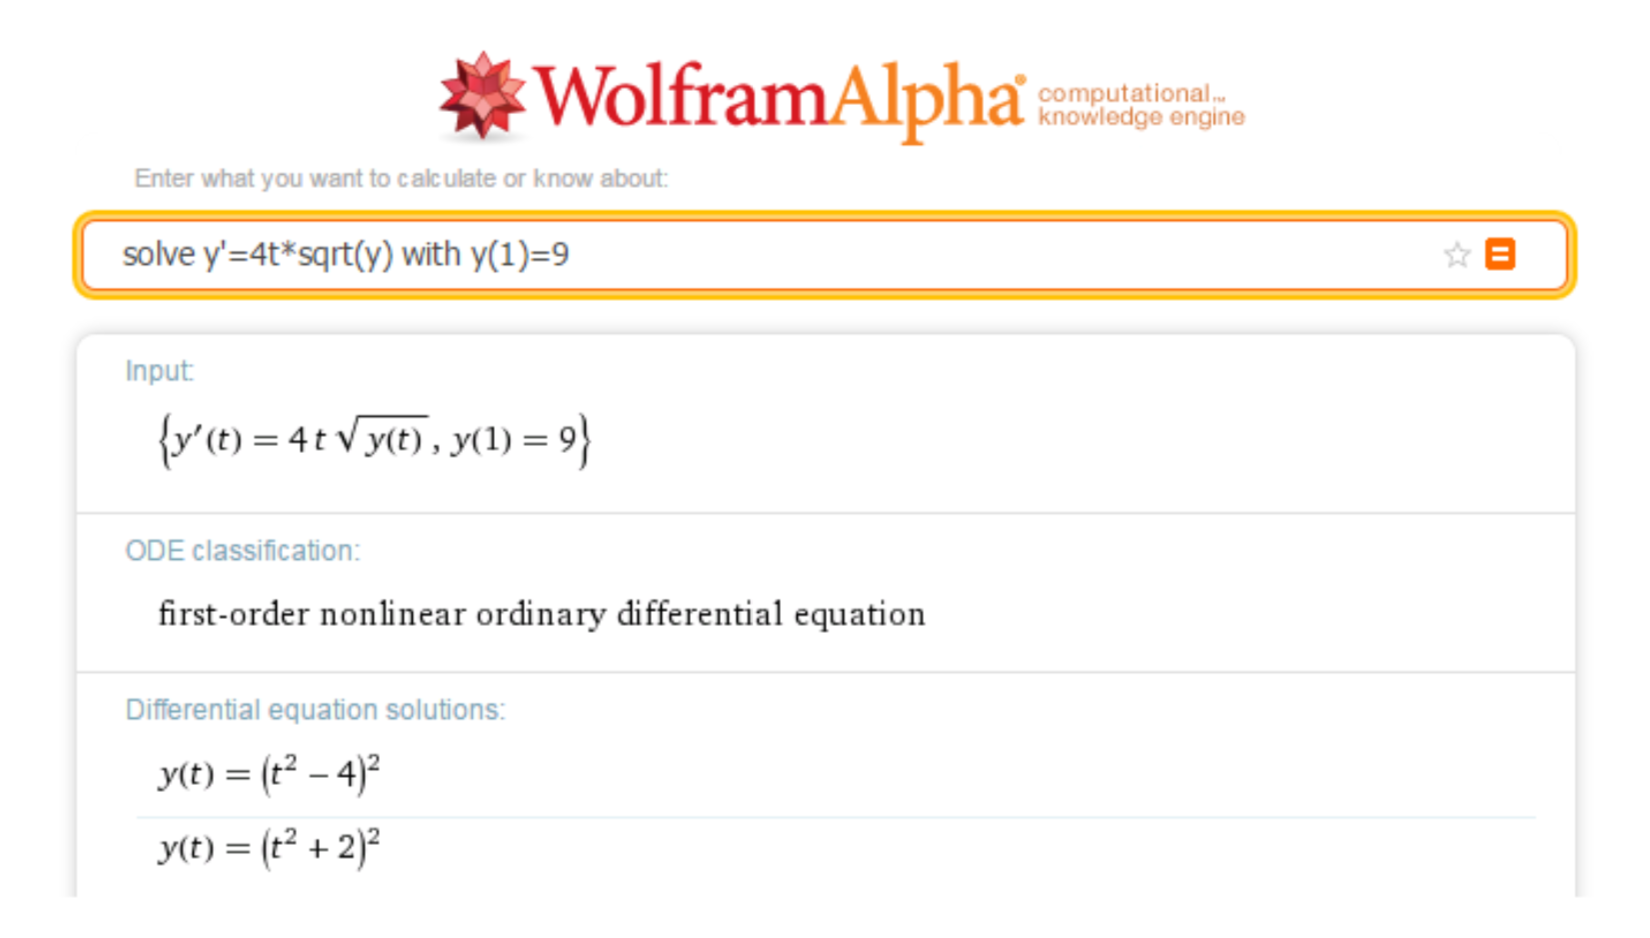
\includegraphics[width=150mm]{5p3.jpg}
\end{figure}

\newpage

%------------------------- Problem 4 -----------------------

\begin{problem}[4]
Here are five physical scenarios that involve oscillations. In each, identify the source of damping (if it is present) that causes oscillations to die out over time, and any relevant forcing (inputs) to the system that might cause it to oscillate.

\begin{enumerate}
\item Tall buildings can sway (with period of motion on the order of a few seconds) 
\item Water sloshing around in a cup
\item Violins, pianos, any stringed instrument 
\item Shock absorbers in a car
\item (Make up your own)
\end{enumerate}
\end{problem}

\newpage

%------------------------- Problem 5 -----------------------

\begin{problem}[5]
Examine Student P’s work on the following problem. What did the student do correctly? What mistake(s) did the student make? What is a more correct response to the problem, and what would you say to help the student understand how to correctly complete the problem?
\end{problem}
\begin{figure}[ht!]
\centering
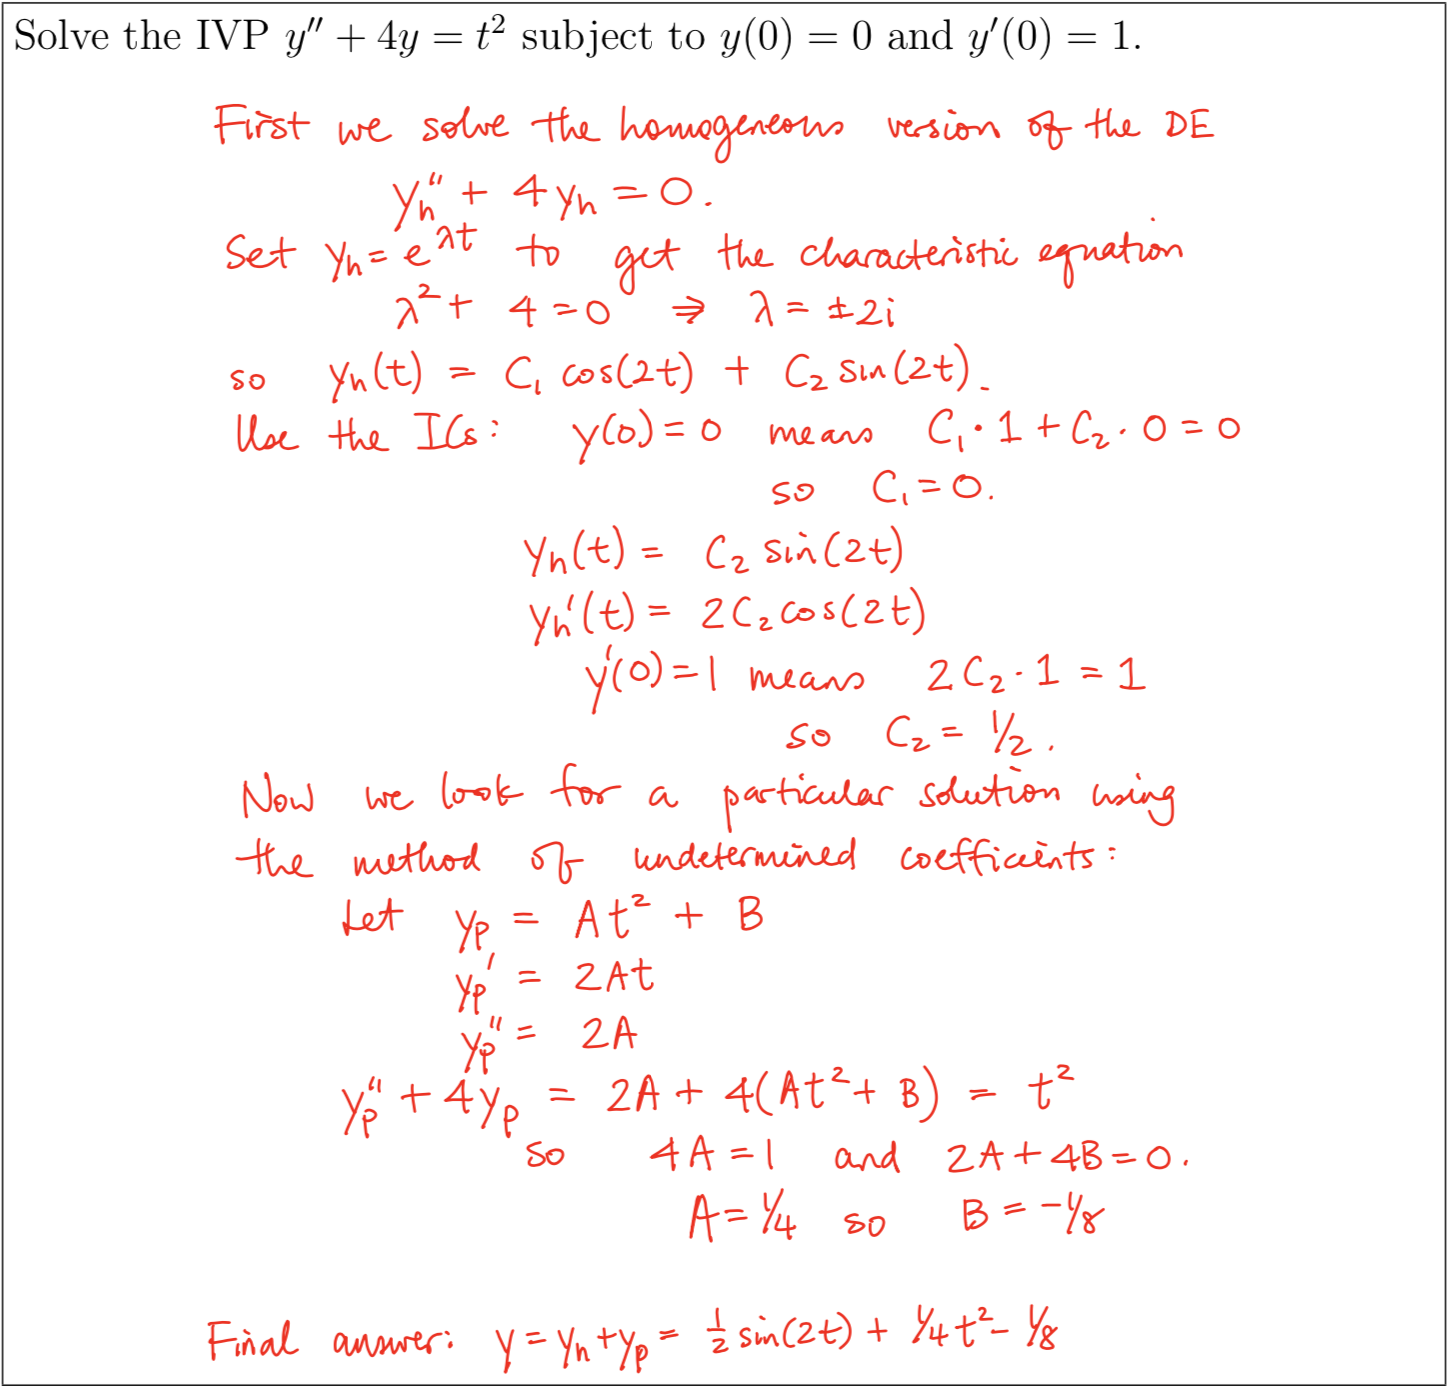
\includegraphics[width=150mm]{6p5.jpg}
\end{figure}

\newpage
\hfill
\newpage
%------------------------- Problem 6 -----------------------

\begin{problem}[6]
\v{Instructions on final project:}\\
• Please continue to work on your Math 45 final project. We suggest each of you put in at least three hours of work into your final project this week. Have every group member sign your homework to demonstrate that you worked together.\\
• Strive to have each person contribute a fair and equitable amount of work and decision- making into the project.\\
• Start thinking ahead about how you want to communicate your findings to the rest of the class. Each group is limited to 10 minutes. (We are allowing time for questions on top of that.) Each person should have a role during the presentation. If you want to create a set of presentation slides, you may find a PowerPoint template in Sakai.
\end{problem}

